\documentclass{article}
\usepackage[francais]{babel}
\usepackage[utf8]{inputenc} % Required for including letters with accents
\usepackage[T1]{fontenc} % Use 8-bit encoding that has 256 glyphs
\usepackage{pythontex}
\usepackage{amsthm}
\usepackage{amsmath}
\usepackage{amssymb}
\usepackage{mathrsfs}
\usepackage{graphicx}
\usepackage{geometry}
\usepackage{stmaryrd}
\usepackage{tikz}
\usetikzlibrary{patterns}
%\usetikzlibrary{intersections}
\usepackage[cache=false]{minted}

\usepackage{stmaryrd}
%\usepackage{tikz}
%\usetikzlibrary{tikzmark}
\usepackage{empheq}
\usepackage{longtable}
\usepackage{booktabs} 
\usepackage{array}
\usepackage{pstricks}
\usepackage{pst-3dplot}
\usepackage{pst-tree}
\usepackage{pstricks-add}
\usepackage{upgreek}
%\usepackage{epstopdf}
\usepackage{eolgrab}
\usepackage{chngpage}
 \usepackage{calrsfs}
 % Appel du package pythontex 
\usepackage{pythontex}

\usepackage{algorithm2e}
\RestyleAlgo{algoruled}
  \SetKw{KwFrom}{from} 
\newenvironment{algo}{
\begin{algorithm}[H]
\DontPrintSemicolon \SetAlgoVlined}
{\end{algorithm}}



\usetikzlibrary{decorations.pathmorphing}
\def \de {{\rm d}}
\usepackage{color}
\usepackage{xcolor}
\newcommand{\mybox}[1]{\fbox{$\displaystyle#1$}}
\newcommand{\myredbox}[1]{\fcolorbox{red}{white}{$\displaystyle#1$}}
\newcommand{\mydoublebox}[1]{\fbox{\fbox{$\displaystyle#1$}}}
\newcommand{\myreddoublebox}[1]{\fcolorbox{red}{white}{\fcolorbox{red}{white}{$\displaystyle#1$}}}

\usepackage{xcolor}
%\setbeamercolor{background canvas}{bg=lightgray}
\usepackage{listings}
\definecolor{purple2}{RGB}{153,0,153} % there’s actually no standard purple
\definecolor{green2}{RGB}{0,153,0} % a
\lstset{%
language=Python, % 
basicstyle=\normalsize\ttfamily, % 
% Color settings to match IDLE style 
keywordstyle=\color{orange}, % 
keywordstyle={[2]\color{purple2}}, % 
stringstyle=\color{green2}, 
commentstyle=\color{red}, 
upquote=true, %
}
\lstdefinestyle{Python}{
    language        = Python,
    basicstyle      = \ttfamily,
    keywordstyle    = \color{blue},
    keywordstyle    = [2] \color{teal}, % just to check that it works
    stringstyle     = \color{violet},
    commentstyle    = \color{red}\ttfamily
}
 \title{Mise en place d'une application symfony}
\author{Ibrahim ALAME}
\date{14/02/2023}
\begin{document}
\maketitle

\section{Création d'une application}  
\subsection{Création d'une application}  
Nous allons utiliser le {\tt CLI} pour créer notre première application. Ouvrez un terminal et commencez par vous placez dans le dossier où vous souhaitez créer l'application, par exemple sur le bureau, puis tapez la commande suivante :
\begin{verbatim}
symfony new dymaproject
\end{verbatim}


Vous aurez ensuite quelque chose comme cela :
\begin{center}
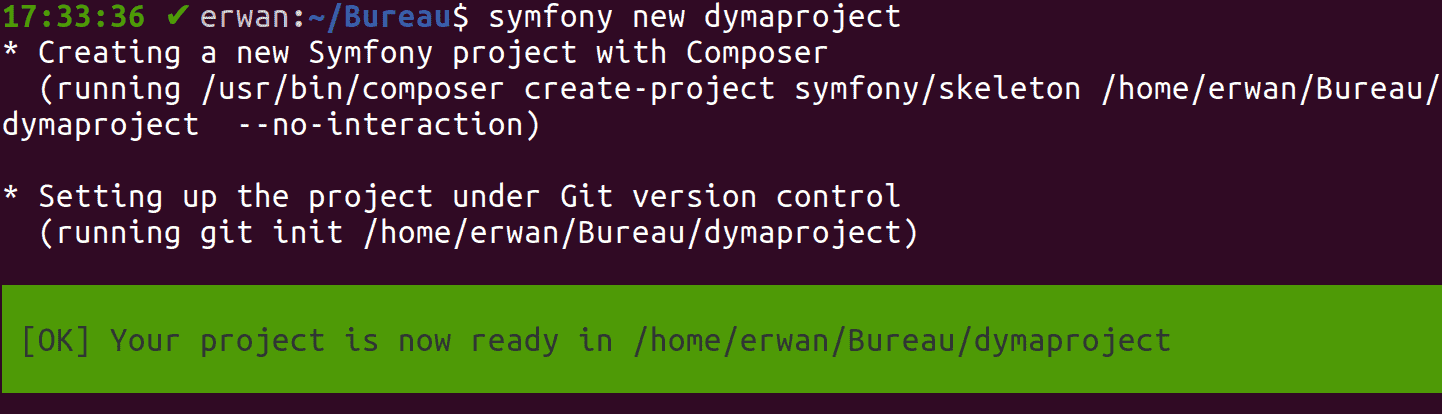
\includegraphics[width=15cm]{images/image1.png}
\end{center}

Ouvrez ensuite le projet dans {\tt Visual Studio Code}.

\subsection{Git par défaut}
Par défaut, {\tt Symfony} utilise Git et crée un premier commit avec les fichiers initiaux. Vous pouvez le voir en faisant :

\begin{verbatim}
git log
\end{verbatim}

Vous aurez par exemple :
\begin{center}
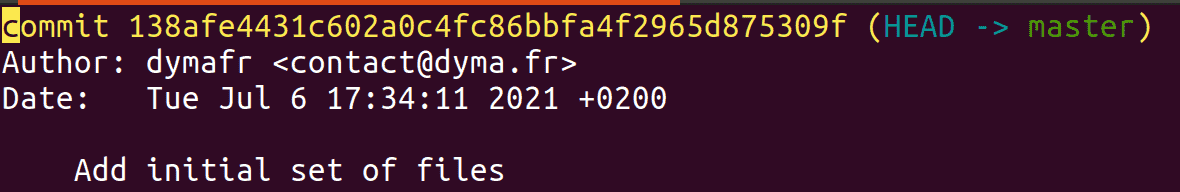
\includegraphics[width=15cm]{images/image2.png}
\end{center}

Lancer le serveur de développement. Pour lancer le serveur de développement local, il suffit d'ouvrir un terminal dans le dossier du projet et de faire :


\begin{verbatim}
symfony serve
\end{verbatim}
Le terminal vous indiquera l'adresse où votre application sera disponible localement :
\begin{center}
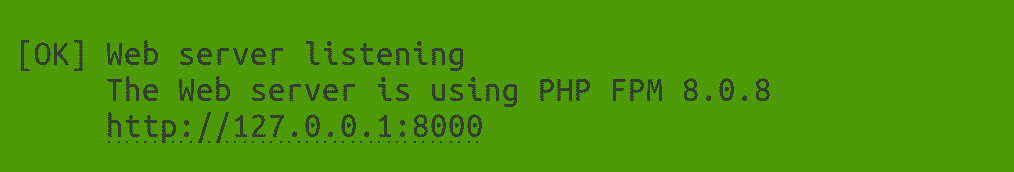
\includegraphics[width=15cm]{images/image3.png}
\end{center}

Vous pouvez couper le serveur à tout moment en faisant {\tt Ctrl + C}.

\subsection{Le fichier {\tt composer.json}}
Le fichier {\tt composer.json} contient toutes les dépendances du projet. Par défaut, {\tt Symfony} en installe plusieurs que nous allons voir ensemble.

\begin{itemize}

\item {\tt symfony/console }: permet de créer des interfaces en ligne de commande plus facilement. C'est le composant utilisé par le CLI Symfony.

\item {\tt symfony/dotenv} : permet d'automatiquement parser les fichiers avec l'extension .env pour charger les variables d'environnement et les rendre disponibles sur {\tt \$\_SERVER} ou {\tt \$\_ENV}.

\item {\tt symfony/flex} : permet de gérer l'architecture des dossiers et fichiers des projets Symfony. Il est utilisé notamment pour générer l'architecture de base lorsque nous avons fait symfony new. Il permet également d'installer de nouvelles dépendances.

\item {\tt symfony/framework-bundle} : librairie qui permet d'intégrer les composants {\tt Symfony} avec le {\tt framework}. Nous verrons que nous utiliserons de nombreux composants.

\item {\tt symfony/runtime} : gère le lancement de {\tt Symfony} quel que soit l'environnement ({\tt PHP-FPM, ReactPHP}, Swoole etc).

\item {\tt symfony/yaml} : permet de parser des fichiers contenant du {\tt YAML} et de les convertir en tableaux associatifs {\tt PHP}.
\end{itemize}


\subsection{Le fichier {\tt .gitignore}}
Nous ne passerons pas trop de temps sur {\tt Git}, nous vous invitons à faire la formation {\tt Git} disponible.

Ce fichier est déjà configuré pour les projets {\tt Symfony} pour ignorer les bons dossiers et fichiers lors des {\tt commit}s.

\subsection{Le fichier .env}
Le fichier .env contient les variables d'environnement.

Ce sont des variables contenant des valeurs nécessaires à l'application pour fonctionne (par exemple des mots de passe ou des secrets pour se connecter à des API tierces etc).

\subsection{Le dossier vendor}
Ce dossier contient toutes les dépendances installées et leurs dépendances en fonction du fichier {\tt composer.json}.

\subsection{Le dossier var}
\begin{itemize}
\item Le dossier {\tt var/cache} contient le système de cache de Symfony. Toute la configuration de l'application est parsée une seule fois et ensuite mise en cache dans ce dossier après le lancement. Cela permet de gagner en performance.

\item Le dossier {\tt var/logs} contient les logs de l'application. Ce sont des fichiers contenant toutes les informations sur les requêtes et les éventuelles erreurs. C'est très utile pour le débogage.
\end{itemize}
\subsection{Le dossier src}
Le dossier {\tt src} pour source contient le code de votre application. Par défaut, il contient la classe {\tt Kernel} (noyau) dans le fichier {\tt Kernel.php}. C'est le point d'entrée dans l'application : il va charger toutes les configurations de l'application.

\subsection{Le dossier public}
Le dossier {\tt public} contient tous les ressources statiques ou {\tt assets} (images, vidéos etc) et le point d'entrée {\tt index.php}.

\subsection{Le dossier config}
\begin{itemize}
\item Le dossier {\tt config} contient la configuration de l'application.

\item Le fichier {\tt routes.yaml} permet de configurer des routes.

\item Le fichier {\tt services.php} contient la configuration des services. Nous étudierons bien sûr les services en détail.

\item Le fichier {\tt bundles.php} permet d'activer ou de désactiver des packages. Les packages ou bundles sont des fonctionnalités utilisables directement dans l'application (c'est équivalent aux modules dans d'autres frameworks).\textbf{•}
\end{itemize}


\subsection{Le dossier bin}
Le dossier bin (pour binaries) contient les fichiers exécutables.


\section{Les composants Symfony}
Les composants Symfony sont des librairies PHP utilisables dans tout environnement PHP (donc pas forcément qu'avec Symfony).

Ces composants sont utilisés dans de très nombreux frameworks et projets PHP. Quelques exemples : bien sûr Symfony, PrestaShop, Drupal,

Nous allons prendre quelques exemples :
\begin{itemize}
\item {\tt Validator} : composant permettant de valider facilement les classes PHP.

\item {\tt Uid} : permet de gérer les identifiants uniques (UUIDs).

\item {\tt Serializer} : permet de transformer des entités dans un format spécifique (JSON ou YAML par exemple) et de désérialiser depuis ces formats vers des entités PHP.

HttpClient, HttpKernel et HttpFoundation : composants pour gérer les requêtes HTTP entrantes et les réponses HTTP sortantes.

\item {\tt Form} : permet de créer et de gérer des formulaires de manière simplifiée.

\end{itemize}

Il y a en tout une soixantaine de composants maintenus par l'équipe Symfony. Nous les verrons au fur et à mesure de nos besoins dans la formation.

\section{Les bundles Symfony}
Les bundles, contrairement aux composants, ne sont utilisables que dans le framework Symfony. Ils sont soit créés et maintenus par l'équipe Symfony, soit par des entités tiers. Ils sont alors appelés des bundles tiers (third-party bundles).

Un bundle permet d'ajouter une fonctionnalité à votre application. Symfony appelle les bundles également des packages, comme nous l'avons vu dans la leçon précédente.

Dans d'autres frameworks, les bundles sont appelés modules ou plugins. Prenons également quelques exemples :

\begin{itemize}
\item {\tt symfony/twig-bundle} : permet d'utiliser Twig de manière optimale avec Symfony. Twig est le moteur de templates pour créer les vues utilisé avec Symfony.

\item {\tt doctrine/doctrine-bundle} : même chose pour Doctrine. Doctrine est un ORM (couche d'abstraction à la base de données) pour PHP.

\item {\tt symfony/swiftmailer-bundle} : permet de gérer les envois d'emails avec les principaux services (Mandrill, SendGrid, Amazon SES etc).

\end{itemize}
Il y a bien sûr beaucoup d'autres bundles Symfony que nous utiliserons au fur et à mesure.

\section{Fonctionnement d'une application Symfony}
Nous allons brièvement voir dans l'ordre les éléments qui gèrent une requête HTTP entrante d'un client :
\begin{center}
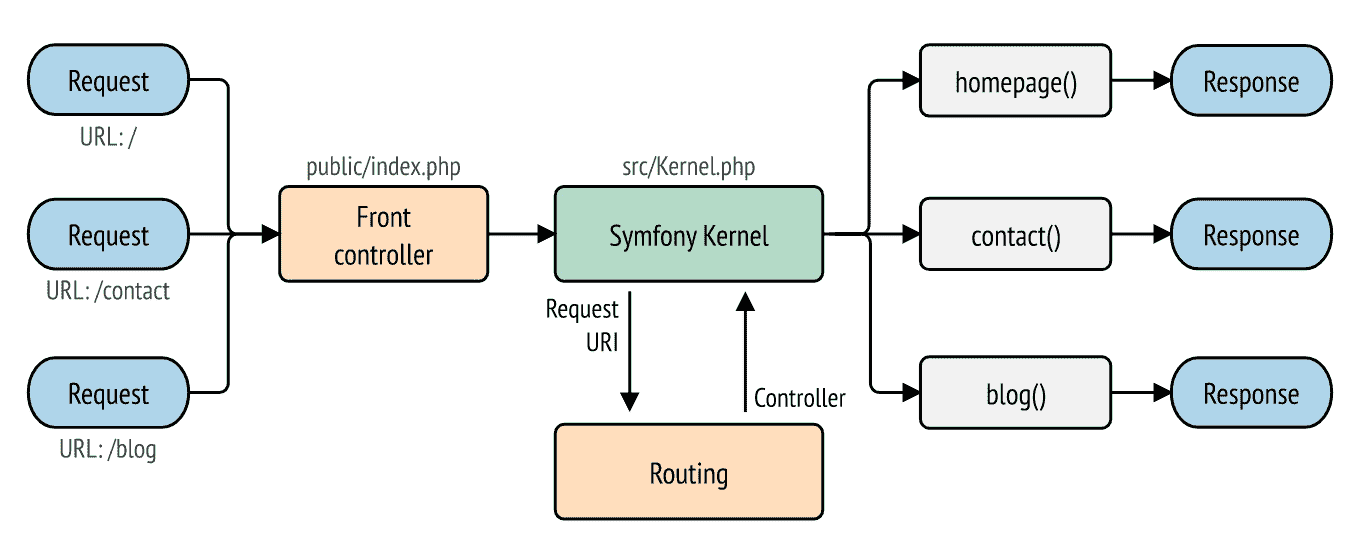
\includegraphics[width=15cm]{images/image4.png}
\end{center}

\subsection{Le script index.php}
Lorsqu'une requête HTTP est reçue par le serveur Web (par exemple NGINX) puis transmise à PHP-FPM (grâce au protocole FastCGI), le premier script PHP à être exécuté est {\tt public/index.php}. On l'appelle point d'entrée ou Front controller.

Le front controller est le contrôleur qui gère l'ensemble des requêtes d'une application. Autrement dit, toutes les requêtes HTTP entraînent obligatoirement l'exécution de ce script.

Si vous avez suivi le cours PHP vous noterez que c'est déjà une différence avec une application PHP basique qui exécute un script différent suivant la requête HTTP et qui n'a donc pas un seul point d'entrée pour l'ensemble des requêtes.

Voici son contenu :
\begin{minted}[
mathescape,
framesep=2mm,
baselinestretch=1.2,
fontsize=\footnotesize,
linenos
]{php}
<?php

use App\Kernel;

require_once dirname(__DIR__).'/vendor/autoload_runtime.php';

return function (array $context) {
    return new Kernel($context['APP_ENV'], (bool) $context['APP_DEBUG']);
};
\end{minted}




Ce script commence par initialiser la fonctionnalité du chargement automatique en fonction de l'environnement (autoload).

Ce script crée ensuite une instance de la classe Kernel.

\subsection{La classe Kernel}
La classe Kernel est chargée par le script index.php, elle se trouve dans src/kernel.php.

Voici son contenu :
\begin{minted}[
mathescape,
framesep=2mm,
baselinestretch=1.2,
fontsize=\footnotesize,
linenos
]{php}
<?php

namespace App;

use SymfonyBundleFrameworkBundleKernelMicroKernelTrait;
use SymfonyComponentHttpKernelKernel as BaseKernel;

class Kernel extends BaseKernel
{
    use MicroKernelTrait;
}
\end{minted}

{\tt Symfony\\Component\\HttpKernel\\Kernel} qui est ici renommée en {\tt BaseKernel} est le cœur de Symfony. Elle va initialiser tous les {\tt bundles Symfony} avec la configuration de votre application.

Vous pouvez aller regarder les fonctions d'initialisation des bundles dans {\tt dymaproject/vendor/symfony/http-kernel/Kernel.php}

Vous y trouverez notamment une fonction initializeBundles() qui est chargée de cette initialisation.

\subsection{La fonction handle()}
Une fois toutes les configurations, le routing et les bundles chargés, la requête est gérée par la fonction {\tt handle()} de la classe {\tt HttpKernel}.

Cette fonction a pour objectif de partir d'une requête HTTP et de la transformer en la réponse HTTP attendue.

C'est donc une fonction très importante dont le schéma suivant résume son fonctionnement :
\begin{center}
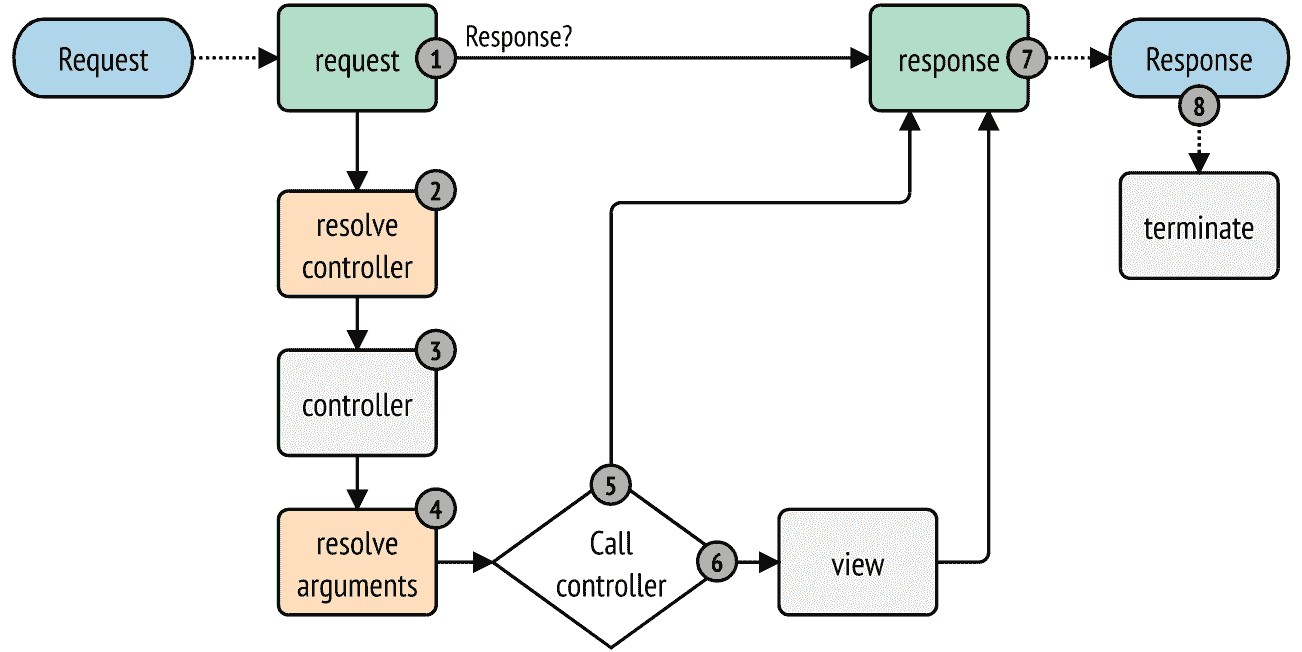
\includegraphics[width=15cm]{images/image5.png}
\end{center}

Cette fonction va envoyer des événements qui sont ensuite gérés par des gestionnaires d'événements.

Nous allons voir les grandes étapes du processus :

\begin{enumerate}
\item Un événement kernel.request est émis. Plusieurs gestionnaires sont appelés à ce niveau. Par exemple, le gestionnaire du bundle Security qui va déterminer si la requête est autorisée ou non. La requête peut être transformée en réponse 403 (pour forbidden) et retournée à ce moment. Un autre gestionnaire important pour cet événement est le Router, il va déterminer quel contrôleur doit être appelé en fonction de la requête.

\item  Le Contrôleur est résolu. La fonction handle() va appeler une fonction getController() (située dans {\tt dymaproject/vendor/symfony/http-kernel/Controller/ControllerResolver.php}) qui va être chargé de récupérer et d'exécuter le bon contrôleur en fonction de la propriété \_controller qui a été placé par le Router sur le tableau associatif Request.

Vous pouvez voir cette mécanique au début de la fonction getController() :
\begin{minted}[
mathescape,
framesep=2mm,
baselinestretch=1.2,
fontsize=\footnotesize,
linenos
]{php}
<?php
public function getController(Request $request) {
  if (!$controller = $request->attributes->get('_controller')) {
    if (null !== $this->logger) {
      $this->logger->warning('Unable to look for the controller as the "_controller" parameter is missing.');
    }
    return false;
  }
}
\end{minted}
\item  Un événement kernel.controller est émis. Il permet d'exécuter des gestionnaires d'événement juste avant que le contrôleur récupéré ne soit exécuté. C'est un design pattern commun appelé hooks en programmation. Cela permet d'exécuter du code lors d'événements clés.

\item  Récupération des arguments pour le contrôleur. Avant l'exécution du contrôleur, une fonction getArguments() va récupérer les arguments à passer au contrôleur en fonction de l'environnement et de la configuration.

\item  Exécution du contrôleur. Le contrôleur, qui est chargé de construire la réponse à renvoyer au client, est exécuté. Il va créer une réponse qui peut être une page HTML, une réponse au format JSON ou toute autre réponse HTTP valide. C'est à cette étape que sera exécuté votre code : votre contrôleur, qui va éventuellement appeler vos modèles et vos vues.

\item  Un événement {\tt kernel.view} est émis. Permet de gérer les cas où aucune réponse n'est retournée par le contrôleur. Par défaut, Symfony n'a aucune gestionnaire pour cet événement et vos contrôleurs doivent obligatoirement retourner une réponse. Certains bundles utilisent cet événement, comme par exemple {\tt FOSRestBundle}.

\item  Un événement {\tt kernel.response} est émis. Permet d'exécuter des gestionnaires juste avant que la réponse ne soit envoyée au client. Des exemples d'utilisation sont la modification des headers de la réponse, l'ajout de cookies etc.

\item  Un événement {\tt kernel.terminate} est émis. La réponse a été envoyée au client. Cet événement permet de procéder aux nettoyages ou à des tâches pouvant être réalisées après la réponse HTTP (par exemple, enregistrement de données d'analyse, envoi d'emails etc).
\end{enumerate}


\section{Création d'une première page}
\subsection{Utiliser HTTPS en local}
Lorsque vous exécutez symfony serve, vous aurez l'avertissement suivant :
\begin{center}
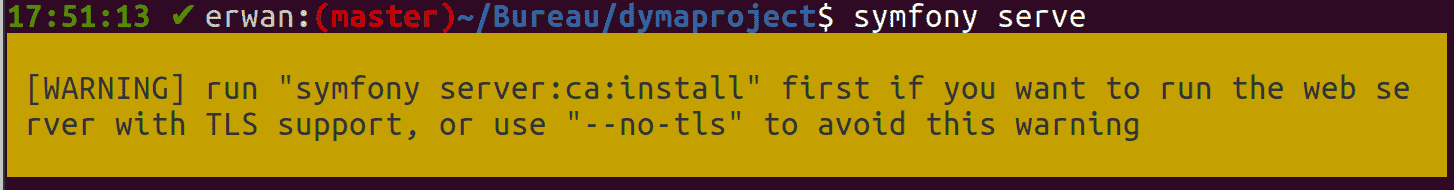
\includegraphics[width=15cm]{images/image6.png}
\end{center}

Il signifie que par défaut, votre serveur de développement local utilisera le protocole HTTP et non sa version sécurisée, le protocole {\tt HTTPS} (utilisant le protocole {\tt TLS}).

Ouvrez donc un terminal dans votre projet et entrez :
\begin{verbatim}
symfony server:ca:install
\end{verbatim}

Le {\tt CLI Symfony} créera un certificat local pour pouvoir utiliser localement {\tt HTTPS}. Il l'ajoutera à vos navigateurs automatiquement :
\begin{verbatim}
The local CA is now installed in the system trust store!
The local CA is now installed in the Firefox and/or Chrome/Chromium trust store (requires browser restart)!
\end{verbatim}

Il faudra les redémarrer pour que le certificat soit pris en compte. Ce certificat n'est évidemment valide que lors du développement en local. Vous pouvez ensuite relancer votre serveur de développement :

\begin{verbatim}
symfony serve
\end{verbatim}

Il sera cette fois disponible par défaut à l'adresse {\tt https://127.0.0.1:8000/}.

Notez bien l'utilisation du protocole {\tt HTTPS} dans {\tt l'URL}.

\subsection{Le langage {\tt YAML}}
Le {\tt YAML} (pour YAML Ain't Markup Language ou "YAML n'est pas un langage de balisage") est un langage permettant de représenter des informations élaborées tout en conservant une grande lisibilité. Il repose principalement sur l'indentation.

C'est un langage utilisé le plus souvent pour des fichiers de configuration.

Nous allons voir les principaux éléments de la syntaxe de ce langage car tout ce que nous verrons à partir de maintenant utilisera du {\tt YAML} :

\# permet de commenter une ligne s'il est placé au début d'une ligne. S'il est avant une chaîne de caractère, il signifie nombre littéral.

$\sim$ signifie valeur nulle.

$-$ permet de créer des listes. Chaque élément d'une liste doit être précédé par - puis un espace. Il doit y avoir un élément par ligne.

clé: valeur permet de déclarer un map clé / valeur.

L'indentation par des espaces permet de créer une hiérarchie, par exemple :

\begin{minted}[
mathescape,
framesep=2mm,
baselinestretch=1.2,
fontsize=\footnotesize,
linenos
]{yaml}
paul:
  nom: Paul Dupont
  emploi: Developer
\end{minted}

Une structure plus complexe :
\begin{minted}[
mathescape,
framesep=2mm,
baselinestretch=1.2,
fontsize=\footnotesize,
linenos
]{yaml}
- paul:
    nom: Paul Dupont
    emploi: Developer
    languages:
      - javascript
      - css
      - html
      - php
\end{minted}

\subsection{Le fichier {\tt config/routes/routes.yaml}}
Dans {\tt Symfony}, vous pouvez écrire des routes directement dans les contrôleurs, comme nous le verrons, ou dans des fichiers {\tt YAML}, {\tt XML} ou {\tt PHP}.

Depuis {\tt Symfony 5.1} seules les routes dans des fichiers écrits en {\tt YAML} sont chargées par défaut. Nous ne verrons donc pas les routes écrites en XML et PHP qui ne sont plus recommandées.

Par défaut, le fichier de route chargé est {\tt config/routes/routes.yaml} :
\begin{minted}[
mathescape,
framesep=2mm,
baselinestretch=1.2,
fontsize=\footnotesize,
linenos
]{yaml}
controllers:
    resource:
        path: ../src/Controller/
        namespace: App\Controller
    type: attribute
\end{minted}

\begin{itemize}
\item {\tt controllers} indique le début de la configuration des contrôleurs.

\item {\tt resource} est utilisée pour déterminer la source des contrôleurs, c'est-à-dire où les fichiers contenant les contrôleurs sont situés.

path spécifie le chemin du répertoire où les fichiers des contrôleurs sont situés. Dans ce cas, les contrôleurs sont stockés dans le dossier Controller du répertoire src.

\item {\tt namespace} spécifie le namespace PHP des contrôleurs. Les namespaces PHP sont utilisés pour organiser et regrouper les classes de manière logique, évitant ainsi les conflits de noms entre les classes. Ici, le namespace des contrôleurs est {\tt App\\Controller}.

\item {\tt type: attribute} indique que les contrôleurs sont définis en utilisant des attributs PHP (disponibles à partir de PHP 8.0). Les attributs permettent d'ajouter des métadonnées à une classe, une méthode ou une propriété. Dans le contexte de Symfony, les attributs sont utilisés pour définir des informations sur le routage, telles que l'URL d'une route et la méthode HTTP associée.

\end{itemize}

Modifiez le fichier {\tt config/routes/routes.yaml} pour ajouter une route pour notre premier contrôleur :
\begin{minted}[
mathescape,
framesep=2mm,
baselinestretch=1.2,
fontsize=\footnotesize,
linenos
]{yaml}
controllers:
    resource:
        path: ../src/Controller/
        namespace: App\Controller
    type: attribute

index:
  path: /
  controller: App\Controller\DefaultController::index
\end{minted}

\begin{itemize}
\item {\tt index} est le nom de la route.

\item {\tt path} est le chemin de la route qui va matcher avec l'URI de la requête HTTP.

\item {\tt controller} est le chemin vers le contrôleur et l'action à exécuter pour la route. Par exemple ici, la classe contrôleur à exécuter est DefaultController, qui se situe dans dymaproject/src/Controller. L'action est située après les doubles deux points ::. Elle correspond à la méthode sur la classe contrôleur qui va être exécutée à chaque requête qui correspond à la route.
\end{itemize}

\subsection{Création du contrôleur}
Pour le moment, le contrôleur n'existe pas et vous aurez une page d'erreur lorsque vous irez sur {\tt https://127.0.0.1:8000/}.

\begin{center}
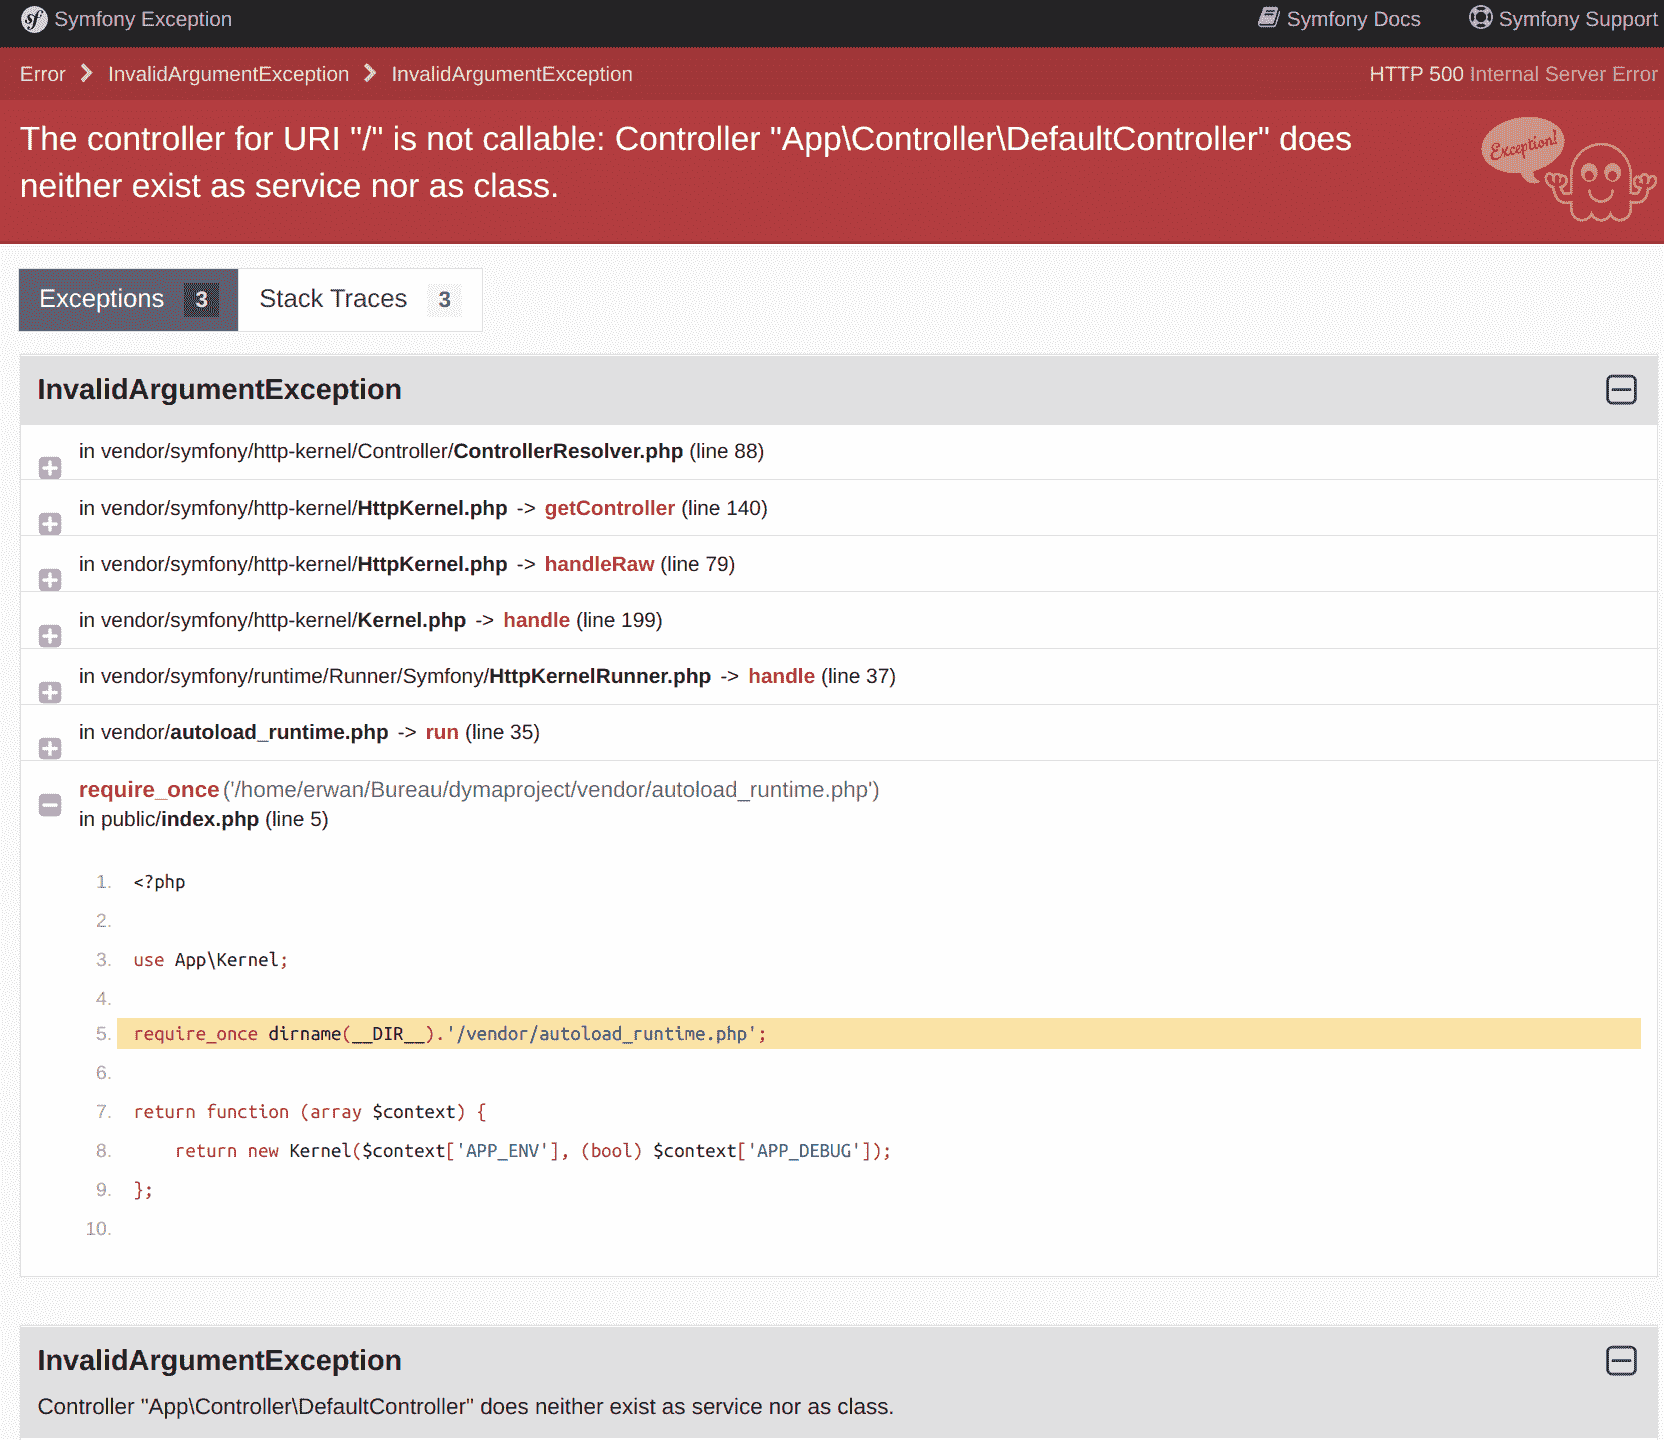
\includegraphics[width=15cm]{images/image7.png}
\end{center}

Notez l'erreur : "Le contrôleur {\tt DefaultController} n'existe pas".

Nous devons donc le créer dans {\tt src/Controller/DefaultController.php} :

\begin{minted}[
mathescape,
framesep=2mm,
baselinestretch=1.2,
fontsize=\footnotesize,
linenos
]{php}
<?php

namespace App\Controller;

use Symfony\Component\HttpFoundation\Response;

class DefaultController
{
  public function index()
  {
    return new Response('<h1>Hello World !</h1>');
  }
}
\end{minted}

Expliquons en détail ce contrôleur.

{\tt namespace App\\Controller;} : permet à la classe d'être importée automatiquement par l'{\tt autoload}. Il faut impérativement commencer par {\tt App} puis respecter le chemin depuis src jusqu'à la classe. Comme notre classe est dans le dossier {\tt src/Controller} il faut donc indiquer {\tt App\\Controller}.

Si vous voulez en savoir plus revoyez les chapitres namespace et Composer et autoload dans la formation PHP.

Nous devons ensuite déclarer la classe en respectant le nom donné dans la route sur la propriété {\tt controller}. Dans notre cas, il faut donc obligatoirement appeler la classe {\tt DefaultController}.

Il faut ensuite créer une méthode sur la classe qui correspond au nom de l'action déclarée sur la route. Dans notre cas l'action est index. Nous devons donc créer une méthode {\tt index()} qui sera exécutée.

Dans cette méthode, nous devons obligatoirement retourner une réponse. Comme nous l'avons vu, l'objectif d'un contrôleur est de recevoir une requête HTTP et de retourner une réponse HTTP.

Pour créer un objet {\tt Response}, commencez à taper {\tt Resp} et vous aurez l'autocomplétion et l'auto-importation de la classe par {\tt VS Code}.


\section{L'objet {\tt Request} du composant {\tt HttpFoundation}}
\subsection{Le composant {\tt HttpFoundation}}
En {\tt PHP}, vous savez qu'il existe un ensemble de variables globales. Par exemple : {\tt \$\_SERVER}, {\tt \$\_GET} ou {\tt \$\_COOKIE}. Le composant {\tt Symfony HttpFoundation} permet de remplacer ces variables globales par des objets, et notamment par {\tt Request} et {\tt Response}.

\subsection{L'objet {\tt Request}}
Pour créer un objet {\tt Request}, il suffit de faire :
\begin{minted}[
mathescape,
framesep=2mm,
baselinestretch=1.2,
fontsize=\footnotesize,
linenos
]{php}
<?php
use Symfony\Component\HttpFoundation\Request;

$request = Request::createFromGlobals();
\end{minted}

La méthode statique {\tt createFromGlobals()} permet de créer l'objet en passant la plupart des variables globales PHP à une méthode {\tt createRequestFromFactory()} :
\begin{minted}[
mathescape,
framesep=2mm,
baselinestretch=1.2,
fontsize=\footnotesize,
linenos
]{php}
public static function createFromGlobals()
{
  $request = self::createRequestFromFactory($_GET, $_POST, [], $_COOKIE, $_FILES, $_SERVER);

  if (0 === strpos($request->headers->get('CONTENT_TYPE', ''), 'application/x-www-form-urlencoded')
    && \in_array(strtoupper($request->server->get('REQUEST_METHOD', 'GET')), ['PUT', 'DELETE', 'PATCH'])
  ) {
    parse_str($request->getContent(), $data);
    $request->request = new InputBag($data);
  }

  return $request;
}
\end{minted}

Sur l'objet {\tt Request}, nous retrouvons les propriétés suivantes :

\begin{itemize}
\item {\tt request} qui contient les informations de la variable globale {\tt \$\_POST}.

\item {\tt query} qui contient les informations de la variable globale {\tt \$\_GET}.

\item {\tt cookies} qui contient les informations de la variable globale {\tt \$\_COOKIE}.

\item {\tt attributes} qui contient des propriétés propres à l'application.

\item {\tt files} qui contient les informations de la variable globale {\tt \$\_FILES}.

\item {\tt server} qui contient les informations de la variable globale {\tt \$\_SERVER}.

\item {\tt headers} qui contient les informations sur les en-têtes qui se trouvent pour la plupart sur la variable globale {\tt \$\_SERVER}.
\end{itemize}
Tous ces objets sont des instances des classes {\tt ParameterBag,InputBag, FileBag, ServerBag} ou {\tt HeaderBag}.

Ces classes contiennent des méthodes permettant d'accéder aux propriétés et de les modifier. Nous verrons toutes ces méthodes en détail au cours de la formation.

Pour donner un exemple, si nous avons une requête {\tt HTTP GET} avec une {\tt query string}, par exemple {\tt ?name=paul} :

\begin{minted}[
mathescape,
framesep=2mm,
baselinestretch=1.2,
fontsize=\footnotesize,
linenos
]{php}
<?php

$request->query->get('name');
\end{minted}
Permet d'accéder à la valeur de la {\tt query string name} et donc ici de retourner {\tt paul}.

\subsection{Code de la vidéo}
Créer un nouveau dossier {\tt php}. Dans ce dossier, {\tt installez symfony/var-dumper} et {\tt symfony/http-foundation} :
\begin{verbatim}
composer require symfony/http-foundation symfony/var-dumper
\end{verbatim}

Créez un fichier {\tt index.php} :

\begin{minted}[
mathescape,
framesep=2mm,
baselinestretch=1.2,
fontsize=\footnotesize,
linenos
]{php}
<?php

use Symfony\Component\HttpFoundation\Request;

require __DIR__ . '/vendor/autoload.php';

$request = Request::createFromGlobals();

dump($request);
dd($request->query->get('name'));
\end{minted}
Lancez ensuite le serveur de développement :
\begin{verbatim}
php -S localhost:3000
\end{verbatim}

Rendez-vous sur {\tt http://localhost:3000/}.



\section{L'objet {\tt Response} du composant {\tt HttpFoundation}}
\subsection{L'objet {\tt Response}}
L'objet {\tt Response} permet de créer, modifier et envoyer une réponse {\tt HTTP}.

\subsubsection{Créer une Response}
Étudions son constructeur :

\begin{minted}[
mathescape,
framesep=2mm,
baselinestretch=1.2,
fontsize=\footnotesize,
linenos
]{php}
<?php

public function __construct(?string $content = '', int $status = 200, array $headers = [])
{
  $this->headers = new ResponseHeaderBag($headers);
  $this->setContent($content);
  $this->setStatusCode($status);
  $this->setProtocolVersion('1.0');
}
\end{minted}
Remarquez que tous les arguments sont optionnels et qu'ils ont des valeurs par défaut.
\begin{itemize}
\item Le premier argument est le contenu de la réponse {\tt HTTP}, qui est vide par défaut.
\item Le second argument est le statut de la réponse {\tt HTTP}, qui {\tt 200} pour {\tt OK} par défaut.
\item Le troisième argument est un tableau associatif pour les en-têtes, qui est vide par défaut.

\end{itemize}

Pour créer une réponse vous pouvez donc par exemple faire :

\begin{minted}[
mathescape,
framesep=2mm,
baselinestretch=1.2,
fontsize=\footnotesize,
linenos
]{php}
<?php

$response = new Response(
  'Vous n\’êtes pas autorisé à voir cette page',
  Response::HTTP_FORBIDDEN,
  ['content-type' => 'text/html']
);
\end{minted}

Remarquez que nous utilisons une constante pour le statut, tous les codes de statut sont disponibles sur la classe {\tt Response} :

\begin{minted}[
mathescape,
framesep=2mm,
baselinestretch=1.2,
fontsize=\footnotesize,
linenos
]{php}
<?php
  public const HTTP_CONTINUE = 100;
  public const HTTP_SWITCHING_PROTOCOLS = 101;
  public const HTTP_PROCESSING = 102;            // RFC2518
  public const HTTP_EARLY_HINTS = 103;           // RFC8297
  public const HTTP_OK = 200;
  public const HTTP_CREATED = 201;
  public const HTTP_ACCEPTED = 202;
  public const HTTP_NON_AUTHORITATIVE_INFORMATION = 203;
  public const HTTP_NO_CONTENT = 204;
  public const HTTP_RESET_CONTENT = 205;
  public const HTTP_PARTIAL_CONTENT = 206;
  public const HTTP_MULTI_STATUS = 207;          // RFC4918
  public const HTTP_ALREADY_REPORTED = 208;      // RFC5842
  public const HTTP_IM_USED = 226;               // RFC3229
  public const HTTP_MULTIPLE_CHOICES = 300;
  public const HTTP_MOVED_PERMANENTLY = 301;
  public const HTTP_FOUND = 302;
  public const HTTP_SEE_OTHER = 303;
  public const HTTP_NOT_MODIFIED = 304;
  public const HTTP_USE_PROXY = 305;
  public const HTTP_RESERVED = 306;
  public const HTTP_TEMPORARY_REDIRECT = 307;
  public const HTTP_PERMANENTLY_REDIRECT = 308;  // RFC7238
  public const HTTP_BAD_REQUEST = 400;
  public const HTTP_UNAUTHORIZED = 401;
  public const HTTP_PAYMENT_REQUIRED = 402;
  public const HTTP_FORBIDDEN = 403;
  public const HTTP_NOT_FOUND = 404;
  public const HTTP_METHOD_NOT_ALLOWED = 405;
  public const HTTP_NOT_ACCEPTABLE = 406;
  public const HTTP_PROXY_AUTHENTICATION_REQUIRED = 407;
  public const HTTP_REQUEST_TIMEOUT = 408;
  public const HTTP_CONFLICT = 409;
  public const HTTP_GONE = 410;
  public const HTTP_LENGTH_REQUIRED = 411;
  public const HTTP_PRECONDITION_FAILED = 412;
  public const HTTP_REQUEST_ENTITY_TOO_LARGE = 413;
  public const HTTP_REQUEST_URI_TOO_LONG = 414;
  public const HTTP_UNSUPPORTED_MEDIA_TYPE = 415;
  public const HTTP_REQUESTED_RANGE_NOT_SATISFIABLE = 416;
  public const HTTP_EXPECTATION_FAILED = 417;
  public const HTTP_I_AM_A_TEAPOT = 418;                                               // RFC2324
  public const HTTP_MISDIRECTED_REQUEST = 421;                                         // RFC7540
  public const HTTP_UNPROCESSABLE_ENTITY = 422;                                        // RFC4918
  public const HTTP_LOCKED = 423;                                                      // RFC4918
  public const HTTP_FAILED_DEPENDENCY = 424;                                           // RFC4918
  public const HTTP_TOO_EARLY = 425;                                                   // RFC-ietf-httpbis-replay-04
  public const HTTP_UPGRADE_REQUIRED = 426;                                            // RFC2817
  public const HTTP_PRECONDITION_REQUIRED = 428;                                       // RFC6585
  public const HTTP_TOO_MANY_REQUESTS = 429;                                           // RFC6585
  public const HTTP_REQUEST_HEADER_FIELDS_TOO_LARGE = 431;                             // RFC6585
  public const HTTP_UNAVAILABLE_FOR_LEGAL_REASONS = 451;
  public const HTTP_INTERNAL_SERVER_ERROR = 500;
  public const HTTP_NOT_IMPLEMENTED = 501;
  public const HTTP_BAD_GATEWAY = 502;
  public const HTTP_SERVICE_UNAVAILABLE = 503;
  public const HTTP_GATEWAY_TIMEOUT = 504;
  public const HTTP_VERSION_NOT_SUPPORTED = 505;
  public const HTTP_VARIANT_ALSO_NEGOTIATES_EXPERIMENTAL = 506;                        // RFC2295
  public const HTTP_INSUFFICIENT_STORAGE = 507;                                        // RFC4918
  public const HTTP_LOOP_DETECTED = 508;                                               // RFC5842
  public const HTTP_NOT_EXTENDED = 510;                                                // RFC2774
  public const HTTP_NETWORK_AUTHENTICATION_REQUIRED = 511;
\end{minted}

Cela permet une meilleure lisibilité du code et de ne pas se tromper sur le statut.

\subsubsection{Modifier une {\tt Response}}
La classe possède également des propriétés publiques qui sont modifiables avec des setters.

{\bf Il est ainsi possible de modifier un objet Response une fois que celui-ci a été créé}.

Pour rappel, un setter est une méthode permettant de modifier une propriété sur un objet.

Par exemple, pour modifier le contenu de la réponse :

\begin{minted}[
mathescape,
framesep=2mm,
baselinestretch=1.2,
fontsize=\footnotesize,
linenos
]{php}
<?php
$response->setContent('Hello World !');
\end{minted}

Même chose pour les en-têtes :

\begin{minted}[
mathescape,
framesep=2mm,
baselinestretch=1.2,
fontsize=\footnotesize,
linenos
]{php}
<?php
$response->headers->set('Content-Type', 'text/plain');
\end{minted}
Et pour le code de statut :

\begin{minted}[
mathescape,
framesep=2mm,
baselinestretch=1.2,
fontsize=\footnotesize,
linenos
]{php}
<?php
$response->setStatusCode(Response::HTTP_NOT_FOUND);
\end{minted} 

\subsubsection{Envoyer la Response}
Une fois que l'objet Response est prêt à être envoyé au client, il suffit d'appeler la méthode send() :

\begin{minted}[
mathescape,
framesep=2mm,
baselinestretch=1.2,
fontsize=\footnotesize,
linenos
]{php}
<?php
$response->send();
\end{minted} 

\subsection{Les réponses au format {\tt JSON}}
Bien qu'il soit possible d'utiliser l'objet {\tt Response} pour envoyer une réponse au format {\tt JSON}, ce n'est pas pratique car il faut manuellement définir l'entête {\tt Content-Type} et encoder l'entité {\tt PHP} au format {\tt JSON}.

Le composant {\tt HttpFoundation} a donc une classe spécifique qui permet de faire cela automatiquement pour vous : {\tt JsonResponse}.

Vous pouvez ainsi directement faire :
\begin{minted}[
mathescape,
framesep=2mm,
baselinestretch=1.2,
fontsize=\footnotesize,
linenos
]{php}
<?php
use Symfony\Component\HttpFoundation\JsonResponse;

$response = new JsonResponse(['prenom' => 'Jean' ]);
\end{minted} 

\subsection{Code de la vidéo : dossier {\tt php}}
Dans le fichier {\tt index.php} mettez le code suivant :

\begin{minted}[
mathescape,
framesep=2mm,
baselinestretch=1.2,
fontsize=\footnotesize,
linenos
]{php}
<?php

use Symfony\Component\HttpFoundation\Response;

require __DIR__ . '/vendor/autoload.php';

$response = new Response('<h2>First !</h2><h1>Hello World ! </h1>');

$response->headers->set('salut', 'ca va');

$response->send();
\end{minted} 

Lancez ensuite le serveur de développement :
\begin{verbatim}
php -S localhost:3000
\end{verbatim}

Rendez-vous sur {\tt http://localhost:3000/}.

\subsection{Code de la vidéo : dossier {\tt dymaproject}}
De retour sur le projet {\tt Symfony}, nous modifions notre contrôleur pour récupérer l'objet Request créé par {\tt Symfony} dans l'action index :

\begin{minted}[
mathescape,
framesep=2mm,
baselinestretch=1.2,
fontsize=\footnotesize,
linenos
]{php}
<?php

namespace App\Controller;

use Symfony\Component\HttpFoundation\Request;
use Symfony\Component\HttpFoundation\Response;

class DefaultController
{
  public function index(Request $request)
  {
    dd($request);
    return new Response('<h1>Hello World !</h1>');
  }
}
\end{minted} 

{\tt Symfony} passe automatiquement l'objet {\tt Request}, qu'il créée automatiquement, en argument des actions.

Pour rappel, les actions sont les méthodes sur les classes des contrôleurs qui sont exécutées lorsqu'une requête {\tt HTTP} correspond à une route.

Notez bien la propriété {\tt attributes} sur l'objet requête :

\begin{center}
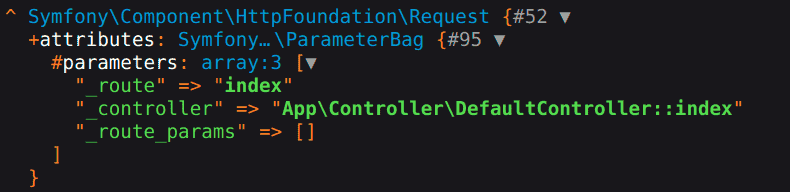
\includegraphics[width=15cm]{images/image8.png}
\end{center}

Comme nous l'avons vu, il s'agit d'une instance de la classe {\tt ParamaterBag} qui contient des paires clé / valeur créées par l'application.

Dans ces paires nous retrouvons, comme prévu, le nom de la route dans {\tt \_route} et le chemin vers le contrôleur, et plus précisément son action, à exécuter dans {\tt \_controler}.

\end{document}




